\documentclass[12pt,letterpaper]{article}
\usepackage[margin=.7in,headheight=18pt,headsep=17pt,footskip=28pt]{geometry}
\usepackage{tikz,fancyhdr,amssymb}
\usetikzlibrary{arrows.meta}
\pdfmapfile{+cm.map}\pdfmapfile{+cmextra.map}\pdfmapfile{+symbols.map}\pdfmapfile{+latxfont.map}
\renewcommand{\familydefault}{\sfdefault}
\setlength{\parindent}{0pt}\setlength{\parskip}{9pt}
\pagestyle{fancy}\fancyhf{}
\fancyhead[L]{\small Week 69 / Thin and fat road triangles / Grades 4--5}
\fancyfoot[L]{\footnotesize Bellingham Math Circle / Week 69 / GGT69-S-v1}
\fancyfoot[R]{\footnotesize\thepage}\renewcommand{\headrulewidth}{.4pt}

\newcommand{\problem}[2]{\par\textbf{Problem #1:} #2\par}
\newcommand{\grid}[1]{\draw[gray!60,line width=.6pt,step=1] (0,0) grid (#1,#1);\foreach \x in {0,...,#1}\foreach \y in {0,...,#1}\fill (\x,\y) circle (1.7pt);}
\newcommand{\home}[3]{\node[draw,circle,fill=white,inner sep=2.5pt,font=\bfseries] at (#1,#2){#3};}
\newcommand{\corners}[1]{\home{0}{0}{A}\home{#1}{0}{B}\home{#1}{#1}{C}}
\newcommand{\treeone}{
\foreach \n/\x/\y in {a/0/0,b/1/0,c/2/0,d/3/0,e/4/1,f/4/-1,g/2/1,h/2/2,i/1/-1,j/0/-1,k/3/2,l/0/1}{\coordinate (\n) at (\x,\y);}
\draw[line width=.9pt] (a)--(b)--(c)--(d)--(e) (d)--(f) (c)--(g)--(h)--(k) (b)--(i)--(j) (a)--(l);
\foreach \n in {a,b,c,d,e,f,g,h,i,j,k,l}\fill (\n) circle (2.6pt);}
\newcommand{\treetwo}{
\foreach \n/\x/\y in {a/0/0,b/1/0,c/2/0,d/3/0,e/4/0,f/1/1,g/0/2,h/2/2,i/3/-1,j/4/-2,k/2/-2}{\coordinate (\n) at (\x,\y);}
\draw[line width=.9pt] (a)--(b)--(c)--(d)--(e) (b)--(f)--(g) (f)--(h) (d)--(i)--(j) (i)--(k);
\foreach \n in {a,b,c,d,e,f,g,h,i,j,k}\fill (\n) circle (2.6pt);}
\begin{document}
Each road between neighboring dots is one step. A shortest route uses the fewest steps. Roads may be drawn at different lengths.

\begin{center}
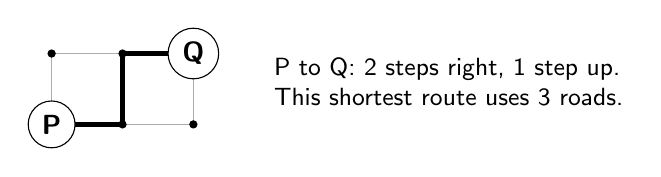
\begin{tikzpicture}[x=.9cm,y=.9cm,font=\small]
\draw[gray!65,step=1] (0,0) grid (2,1);\foreach \x in {0,1,2}\foreach \y in {0,1}\fill (\x,\y) circle (1.5pt);
\draw[line width=2pt] (0,0)--(1,0)--(1,1)--(2,1);\home{0}{0}{P}\home{2}{1}{Q}
\node[anchor=west,align=left] at (3,.6){P to Q: 2 steps right, 1 step up.\\This shortest route uses 3 roads.};
\end{tikzpicture}
\end{center}
For three homes A, B, C, choose a shortest route for each pair. Color AB red, BC blue, and CA green. These three routes are a road triangle. Routes may overlap; draw the colors side by side when they do. Your partner checks that each route is shortest.
\problem{1}{Choose three different dots for the homes on each tree. Draw the road triangles. Swap roles and try new homes. Can you make a road that belongs to exactly one of the three colored routes?}
\vspace{.25in}
\begin{center}
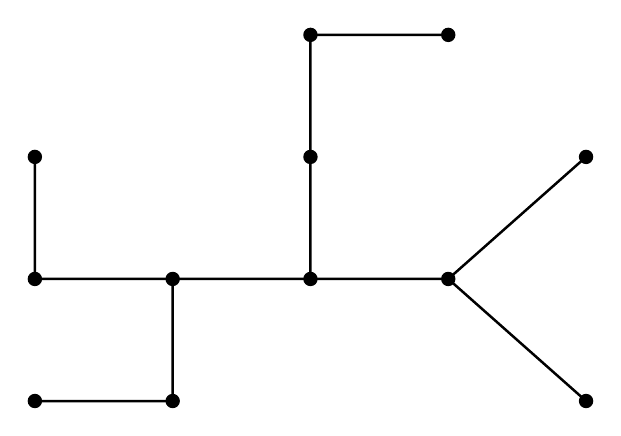
\begin{tikzpicture}[x=1.75cm,y=1.55cm]\treeone\end{tikzpicture}
\vspace{.55in}

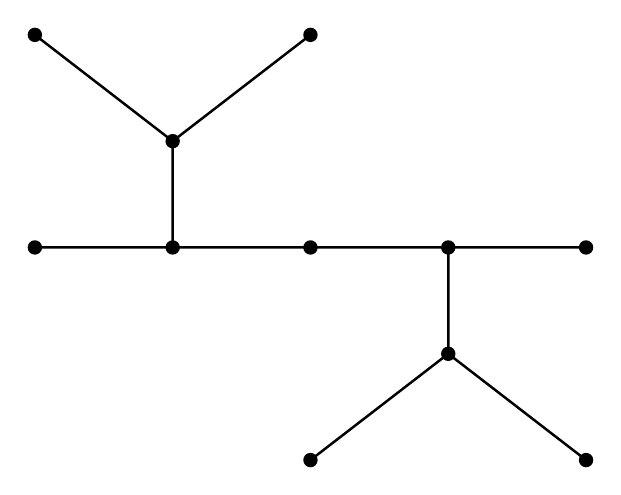
\begin{tikzpicture}[x=1.75cm,y=1.35cm]\treetwo\end{tikzpicture}
\end{center}
\newpage
For a dot on one colored side, its \textbf{gap} is the fewest road steps needed to reach either of the other two colored sides. Use any road on the map, including uncolored roads. A dot already on another side has gap 0.
\begin{center}
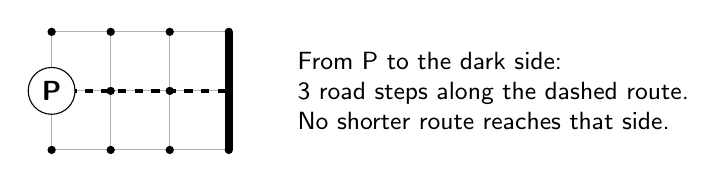
\begin{tikzpicture}[x=.75cm,y=.75cm,font=\small]
\draw[gray!60,step=1] (0,0) grid (3,2);\foreach \x in {0,1,2,3}\foreach \y in {0,1,2}\fill (\x,\y) circle (1.5pt);
\draw[line width=3pt] (3,0)--(3,2);\draw[dashed,line width=1.5pt] (0,1)--(3,1);\home{0}{1}{P}
\node[anchor=west,align=left] at (4,1){From P to the dark side:\\3 road steps along the dashed route.\\No shorter route reaches that side.};
\end{tikzpicture}
\end{center}
\problem{2}{Choose shortest routes for the three sides on each map. Make every gap 0 on one map. On the other, make at least one gap 2 or more. Circle that dot and mark a shortest route to another side. Your partner checks the gap.}
\vspace{.3in}
\begin{center}
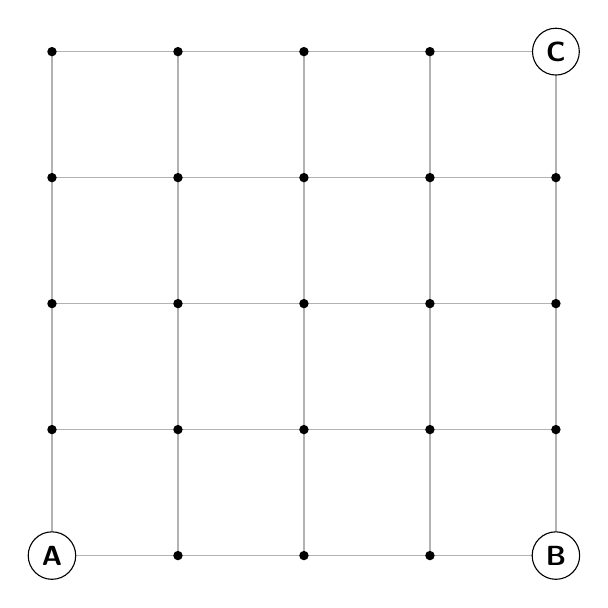
\begin{tikzpicture}[x=1.6cm,y=1.6cm]\grid{4}\corners{4}\end{tikzpicture}\hfill
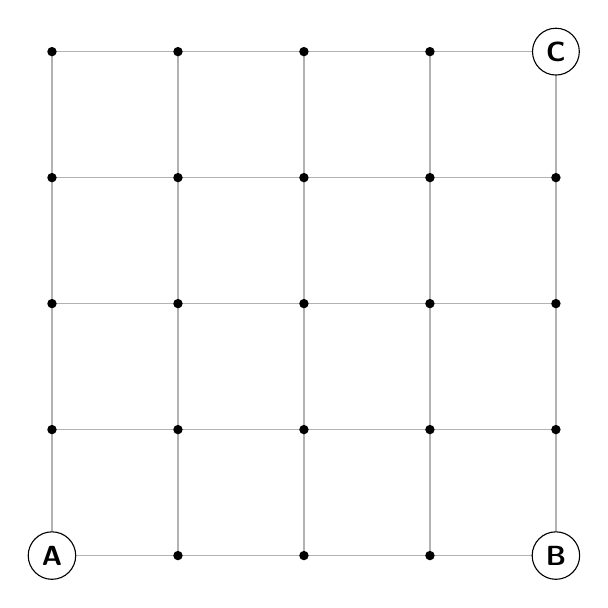
\begin{tikzpicture}[x=1.6cm,y=1.6cm]\grid{4}\corners{4}\end{tikzpicture}
\end{center}
\vspace{.4in}\rule{\linewidth}{.4pt}\par\vspace{.4in}\rule{\linewidth}{.4pt}
\newpage
\problem{3}{On each map, make the biggest gap as large as you can. All three colored sides must be shortest routes. Circle a dot with the biggest gap and write its gap beside it. Your partner tries to find a shorter route from that dot to another side.}
\vspace{.2in}
\begin{center}
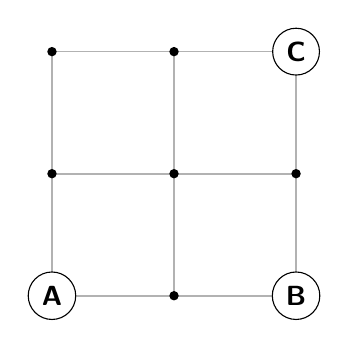
\begin{tikzpicture}[x=1.55cm,y=1.55cm]\grid{2}\corners{2}\end{tikzpicture}\hspace{1.0in}
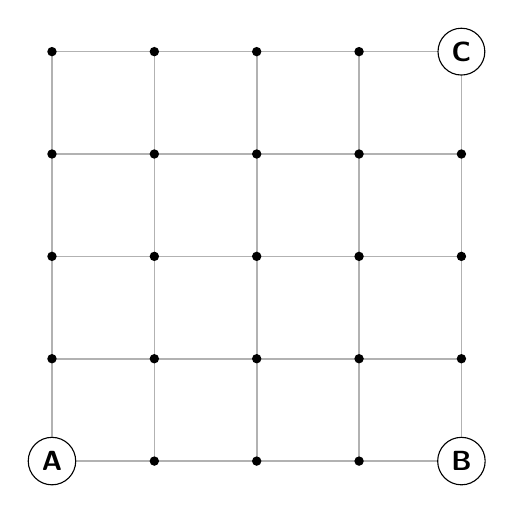
\begin{tikzpicture}[x=1.3cm,y=1.3cm]\grid{4}\corners{4}\end{tikzpicture}
\vspace{.45in}

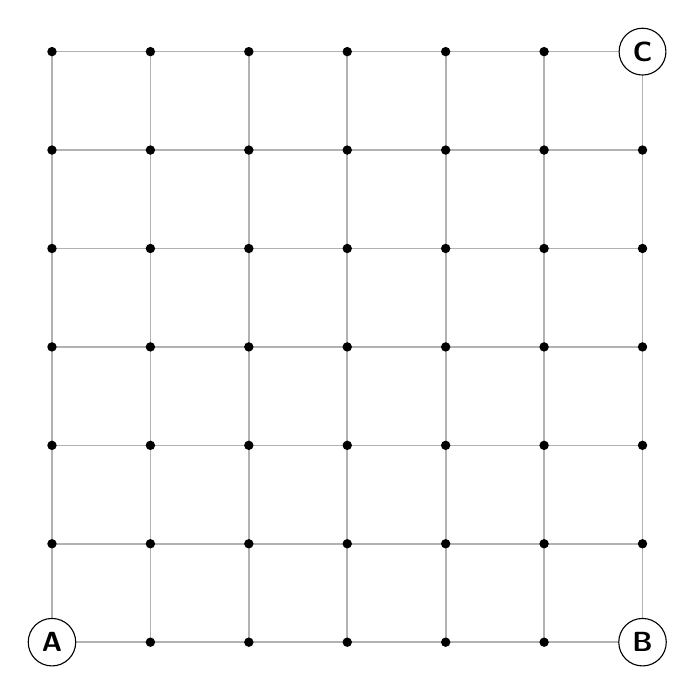
\begin{tikzpicture}[x=1.25cm,y=1.25cm]\grid{6}\corners{6}\end{tikzpicture}
\end{center}
\newpage
\problem{4}{Your partner names a whole number. Make a plan for a square-grid road triangle with a gap bigger than that number. You may use as large a grid as you need. Explain why all three sides are shortest and why your marked dot has the claimed gap.}
\vspace{2.6in}
\rule{\linewidth}{.4pt}\par\vspace{.4in}\rule{\linewidth}{.4pt}
\vspace{.25in}
\problem{5}{A tree is a connected road map with no loops. Can any road triangle on any tree have a positive gap? Explain why your answer holds for every choice of three homes.}
\vspace{1.0in}\rule{\linewidth}{.4pt}\par\vspace{.4in}\rule{\linewidth}{.4pt}\par\vspace{.4in}\rule{\linewidth}{.4pt}
\end{document}
